\documentclass{beamer}[10pt, usepdftitle=false, handout]

\beamertemplatenavigationsymbolsempty

\usepackage[T1]{fontenc}
\usepackage[]{algorithm2e}
\usepackage{multimedia}
\usepackage{gensymb}
\usepackage{textcomp}

%\usepackage[font=small,labelfont=bf]{caption} 

\usetheme{Boadilla}

\title{Basic of Computer Networks 2}
\author[]{Paul Blondel}
\institute[]{CNAM}
\date[]{March 1st, 2019}

\usepackage[style=british]{csquotes}


\def\signed #1{{\leavevmode\unskip\nobreak\hfil\penalty50\hskip1em
  \hbox{}\nobreak\hfill #1%
  \parfillskip=0pt \finalhyphendemerits=0 \endgraf}}

\newsavebox\mybox
\newenvironment{aquote}[1]
  {\savebox\mybox{#1}\begin{quote}\openautoquote\hspace*{-.7ex}}
  {\unskip\closeautoquote\vspace*{1mm}\signed{\usebox\mybox}\end{quote}}


\setbeamertemplate{headline}
{
  \leavevmode%
  \hbox{%
  \begin{beamercolorbox}[wd=1.0\paperwidth,ht=2.25ex,dp=1ex,center]{author in head/foot}%
    \usebeamerfont{author in head/foot}\insertsubsection
  \end{beamercolorbox}}%
  \vskip0pt%
}


\setbeamertemplate{footline}
{
  \leavevmode%
  \hbox{%
  \begin{beamercolorbox}[wd=.5\paperwidth,ht=2.25ex,dp=1ex,center]{author in head/foot}%
    \usebeamerfont{author in head/foot}\insertsection
  \end{beamercolorbox}%
  \begin{beamercolorbox}[wd=.5\paperwidth,ht=2.25ex,dp=1ex,center]{title in head/foot}%
    \usebeamerfont{title in head/foot} \inserttitle \hspace*{2em}  \insertframenumber{} / \inserttotalframenumber\hspace*{2ex} 
  \end{beamercolorbox}}%
  \vskip0pt%
}

\AtBeginSection[]
{
   \begin{frame}
    \tableofcontents[ 
    currentsection] 
   \end{frame}
}

\begin{document}
	{
	\setbeamertemplate{footline}{
  	\leavevmode%
  	\hbox{%
  	\begin{beamercolorbox}[wd=.5\paperwidth,ht=2.25ex,dp=1ex,center]{author in head/foot}%
  	\end{beamercolorbox}%
  	\begin{beamercolorbox}[wd=.5\paperwidth,ht=2.25ex,dp=1ex,center]{title in head/foot}%
  	\end{beamercolorbox}}%
  	\vskip0pt%	
	} 
	\begin{frame}
	\titlepage
	\end{frame}

	\begin{frame}
	
	\begin{aquote}{Tim-Bernes Lee - Creator of the WEB}
I think, in general, it's clear that most bad things come from misunderstanding, and communication is generally the way to resolve misunderstandings — and the Web's a form of communications — so it generally should be good.
	\end{aquote}	
	
	\end{frame}


	\begin{frame}
		\tableofcontents
	\end{frame}
	}

	\addtocounter{framenumber}{-3}

	\section{Data transmission}	
	\subsection{Exchange organization}

    \begin{frame}[label=(first)]
	
	Transmitting information between two computers can be do in multiple ways:
	
	\begin{itemize}
	
	\item{simplex: each computer has one role: emitting data (source) or  receiving data (receptor) 
	\begin{center}	
	\begin{figure}
		
\includegraphics[scale=0.3]{images/2-1.png} 
     	%\vspace*{-0.5em}
		%\caption{Floating gate transistor cell}
	\end{figure}	
	\end{center}	
	}
	\item{half-duplex: computers can alternate their role: once source, once receptor 
	\begin{center}	
	\begin{figure}
		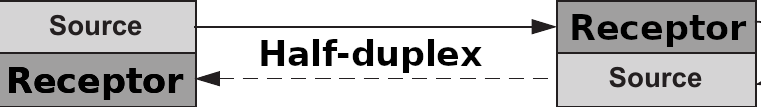
\includegraphics[scale=0.3]{images/2-2.png} 
     	%\vspace*{-0.5em}
		%\caption{Floating gate transistor cell}
	\end{figure}	
	\end{center}	
	}
	\item{full-duplex: computers can send and receive data in the same time 
	\begin{center}	
	\begin{figure}
		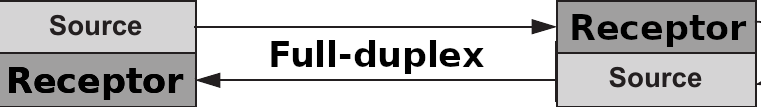
\includegraphics[scale=0.3]{images/2-3.png} 
     	%\vspace*{-0.5em}
		%\caption{Floating gate transistor cell}
	\end{figure}	
	\end{center}	
	}		
	\end{itemize}
	\end{frame}	 
	 
	\subsection{Types of connection}	 
	 
	\begin{frame}
	
	Point-to-point connection:
	\vspace*{1em}
	
	Each computer is linked to only one another.
	
	\begin{center}	
	\begin{figure}
		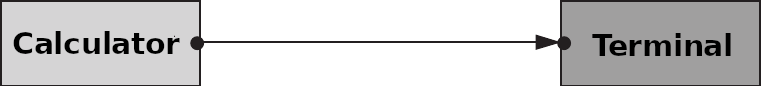
\includegraphics[scale=0.3]{images/2-4.png} 
     	%\vspace*{-0.5em}
		%\caption{Floating gate transistor cell}
	\end{figure}	
	\end{center}
	
	Multiple connections:
	\vspace*{1em}	
	
	Several computers share the same link.
	
	\begin{center}	
	\begin{figure}
		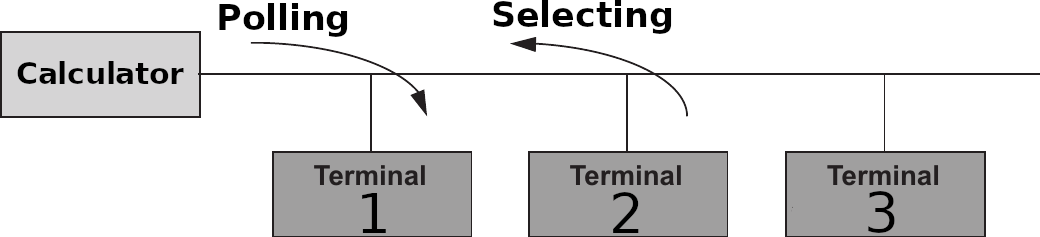
\includegraphics[scale=0.3]{images/2-5.png} 
     	%\vspace*{-0.5em}
		%\caption{Floating gate transistor cell}
	\end{figure}	
	\end{center}
	
	\begin{block}{Notes}
	May have conflicts: it is necessary to control the access! With polling/selecting for instance. 
	\end{block}	
	
	
	\end{frame}	 
	 
	\begin{frame}

	\begin{center}	
	\begin{figure}
		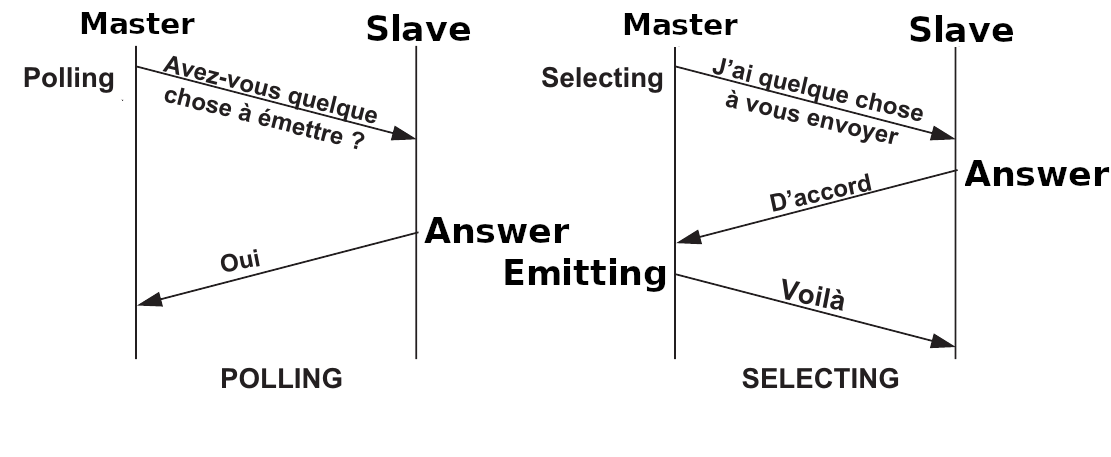
\includegraphics[scale=0.35]{images/2-6.png} 
     	%\vspace*{-0.5em}
		%\caption{Floating gate transistor cell}
	\end{figure}	
	\end{center}
	
	Peer-to-peer communication:
	\vspace*{1em}
	
	\begin{center}	
	\begin{figure}
		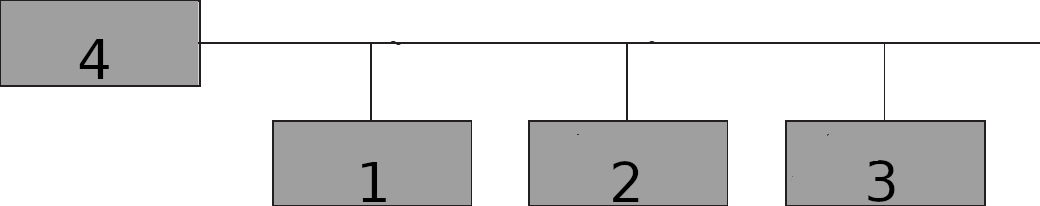
\includegraphics[scale=0.3]{images/2-7.png} 
     	%\vspace*{-0.5em}
		%\caption{Floating gate transistor cell}
	\end{figure}	
	\end{center}	
		
	
	All machines can send towards others calculators: high risk of collisions! Here access policy is decentralized (ex: local networks).	
	
	\end{frame}

	\subsection{Parallel transmission or serial transmission}

	\begin{frame}

	In case the transmission is serial: the link only permit to transmit data bit after bit (like a bus). The bit word is send bit after bit ...
	
	\begin{center}	
	\begin{figure}
		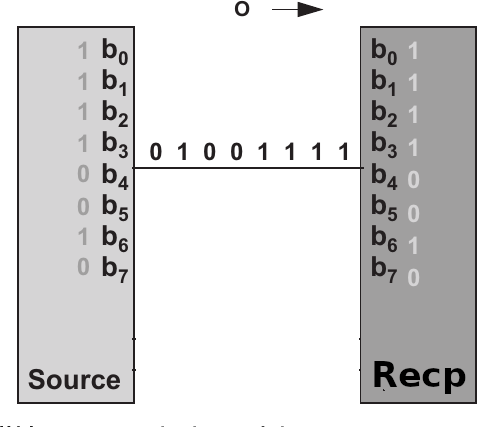
\includegraphics[scale=0.25]{images/2-8.png} 
     	%\vspace*{-0.5em}
		%\caption{Floating gate transistor cell}
	\end{figure}	
	\end{center}	
	
	With parallel transmission: all the bits of the bit word can be send in once.
	
	\begin{center}	
	\begin{figure}
		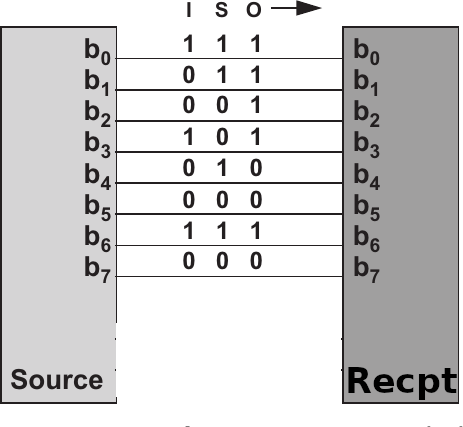
\includegraphics[scale=0.25]{images/2-9.png} 
     	%\vspace*{-0.5em}
		%\caption{Floating gate transistor cell}
	\end{figure}	
	\end{center}	
	
	8 steps to transfer "o" (serial). 1 step to transfer "o" (parallel).
	
	\begin{block}{Notes}
	\begin{itemize}
	\item{Parallel: Faster, but can suffer from delay skew if computers are far one another!}
	\item{Serial: Cheaper and more sure. But it requires an electronic interface to "serialize" and "deserialize" the bits.}
	\end{itemize}	
	\end{block}		
	
	\end{frame}

	\subsection{Synchronous and asynchronous transmissions}
	
	\begin{frame}
	
	All the bits are sent through the link/connection with a certain rhythm (or timing). This rhythm is given by a timer.
	\vspace*{1em}
	
	Both the source and the receptor have timers and they need to be synchronized!
	
	\begin{center}	
	\begin{figure}
		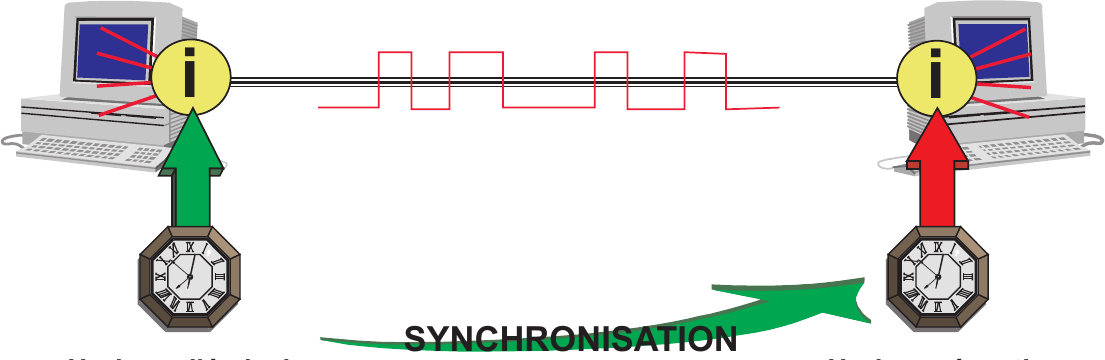
\includegraphics[scale=0.3]{images/2-10.png} 
     	%\vspace*{-0.5em}
		%\caption{Floating gate transistor cell}
	\end{figure}	
	\end{center}
	
	If they are not synchronized: the message might not be correctly received!
	
	\begin{center}	
	\begin{figure}
		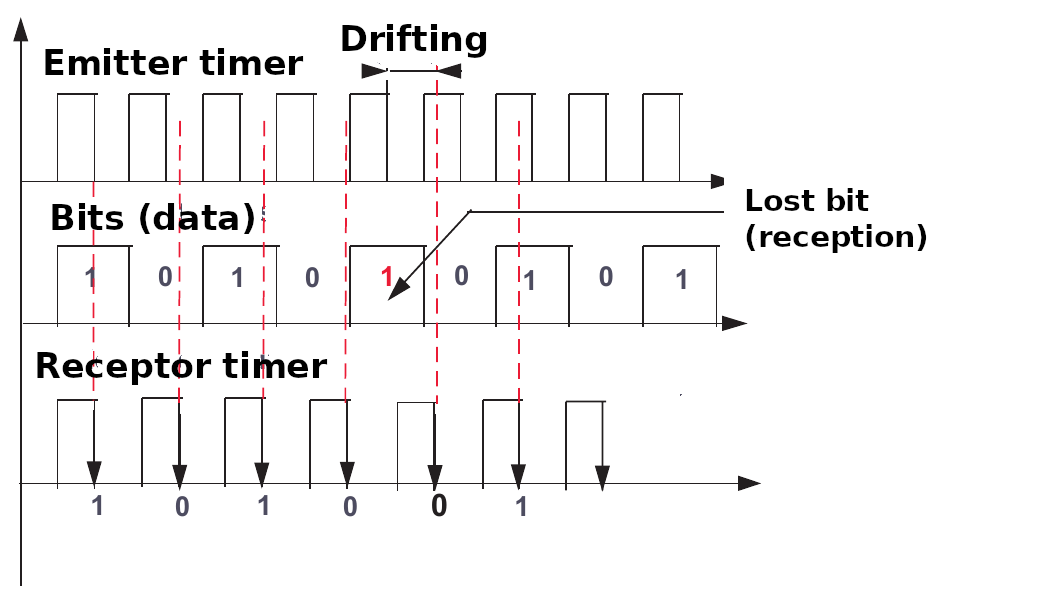
\includegraphics[scale=0.3]{images/2-11.png} 
     	%\vspace*{-0.5em}
		%\caption{Floating gate transistor cell}
	\end{figure}	
	\end{center}
		
	\end{frame}

	\begin{frame}
	
	There are two types of transmissions:
	\vspace*{1em}
	
	\begin{itemize}
	\item{Synchronous transmission (timers are synchronized)}
	\item{Asynchronous transmission (timers are autonomous)}
	\end{itemize}
	\vspace*{1em}

	Synchronous transmission:
	\vspace*{1em}
		
	\begin{itemize}
	\item{A synchronous signal is sent during of the transmission using a specific line.
}
	\item{Or the synchronous signal is deduced from the message itself (more complex to realize)}
	\end{itemize}
	
		
	\begin{block}{Note}
	In both approaches the first bits used to help the synchronization
	
	\end{block}	
	
		
	\end{frame}
	
	\begin{frame}
	
	Asynchronous transmission:
	\vspace*{1em}
	
	Here the timers of the source and the receptor are independent each other (the beginning of the message synchronized the two timers, then timers are let free to drift). 
	\vspace*{0.5em}
	
	The principle of this technique is: there is an interval of time in which the drift (caused by dephasing) does not modify the message.
	\vspace*{0.5em}
	
	This interval of time is big enough to transmit a character (one piece of information).
	
	\begin{center}	
	\begin{figure}
		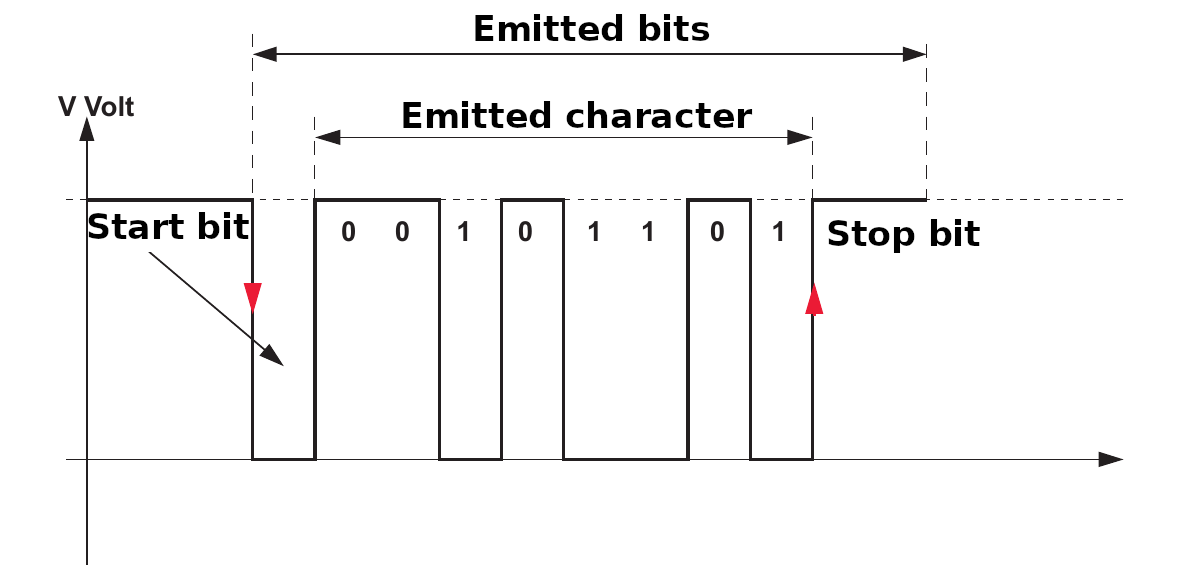
\includegraphics[scale=0.3]{images/2-12.png} 
     	%\vspace*{-0.5em}
		%\caption{Floating gate transistor cell}
	\end{figure}	
	\end{center}
	
	With asynchronous transmission: each character is preceded and followed by delimiters: start and stop bits.	
	
	\end{frame}

	\begin{frame}
	
	Asynchronous transmission: easier approach than synchronous transmission (requiring an explicit synchronization).
	
	\begin{center}	
	\begin{figure}
		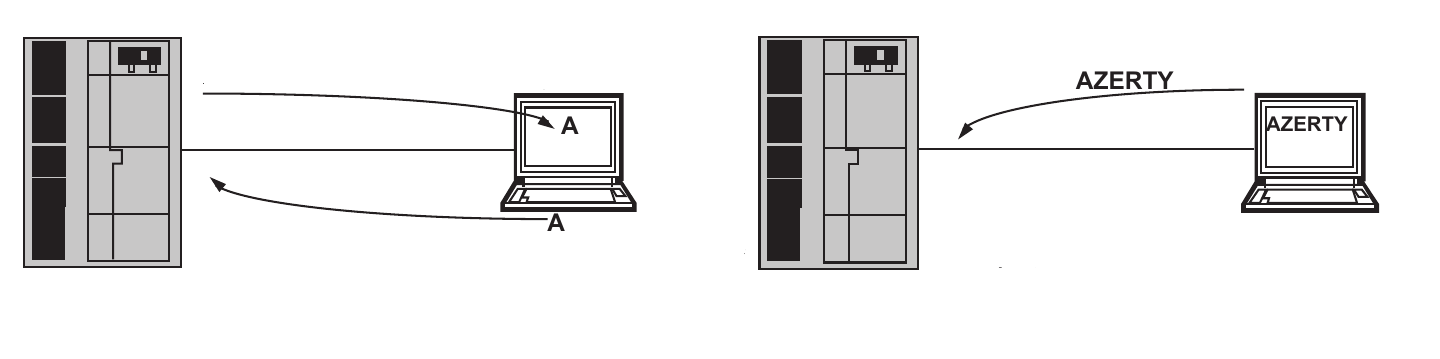
\includegraphics[scale=0.3]{images/2-13.png} 
     	%\vspace*{-0.5em}
		%\caption{Floating gate transistor cell}
	\end{figure}	
	\end{center}
	
	Left: Asynchronous transmission (characters are sent and displayed while the keys are pressed)	
	\vspace*{1em}
	
	Right: Synchronous transmission (all the letters are first buffered then they are sent (word completed) and displayed.	
		
	\end{frame}

	\begin{frame}
	
	Asynchronous transmission: easier but more bits are used for control!
	\vspace*{1em}
	
	Synchronous transmission: optimized but more difficult to make it work.
	
	And asynchronous and synchronous transmission have different usages as well!
	
	\end{frame}

	\begin{frame}
	
	$Eff=\frac{Dr}{Dn}$
	\vspace*{1em}
	
	Dr: number of useful bits that can be transferred	
	
	Dn: total number of bits (control bits included)
	\vspace*{1em}

	$Eff_{Asynchronous\ trans} < Eff_{Synchronous\ trans}$
	
	(For long data transmissions)
		
	
	\end{frame}

	\section{Notions about protocols}

	\begin{frame}
	
	We saw how to transmit data between two computers.
	
	\begin{center}	
	\begin{figure}
		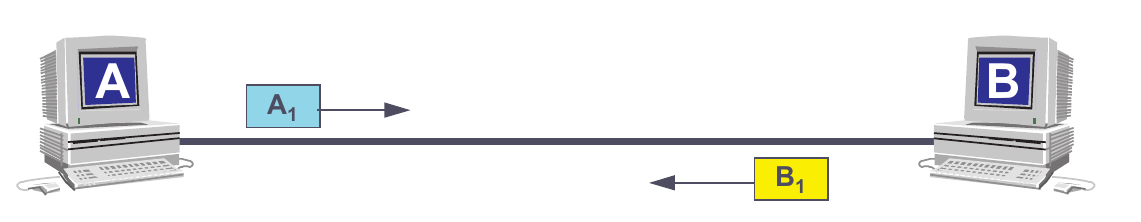
\includegraphics[scale=0.4]{images/2-14.png} 
     	%\vspace*{-0.5em}
		%\caption{Floating gate transistor cell}
	\end{figure}	
	\end{center}
	
	We need a protocol to ensure a reliable exchange of data between the two systems.
	\vspace*{1em}
	
	During the data exchange the protocol ensures:
	\vspace*{0.5em}
	
	\begin{itemize}
	\item{The delimitation of the blocks of exchanged data}
	\item{The control of the integrity of the received data}
	\item{The organization and the control of the exchange}
	\item{Eventually, the control of the link}
	\end{itemize}
		
	\end{frame}

	\subsection{Delimitation of the data}
	
	\begin{frame}
	
	Like in asynchronous transmission where the data is between a "start" and "stop" bit: in synchronous transmission a "flag" delimit the data (to identify the begin and the end of the block).
	\vspace*{1em}
	
	\begin{center}	
	\begin{figure}
		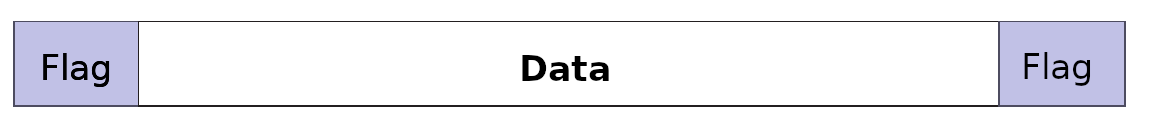
\includegraphics[scale=0.4]{images/2-15.png} 
     	%\vspace*{-0.5em}
		%\caption{Floating gate transistor cell}
	\end{figure}	
	\end{center}
	\vspace*{1em}
	
	The flag is useful for two things:
	\vspace*{0.5em}
	\begin{itemize}
	\item{Delimit data}
	\item{When sent with not data: flags help synchronize the timer of the receptor}	
	\end{itemize}		
	
	
	\end{frame}

	\begin{frame}
	
	The flag is a specific series of bits.	 This series of bits must not be present in the message itself! Otherwise the data will be corrupted.
	\vspace*{1em}
	
	To avoid that: there is the transparency mechanism. This mechanism transforms any flag-like series of bits in the data. 
	
	\begin{center}	
	\begin{figure}
		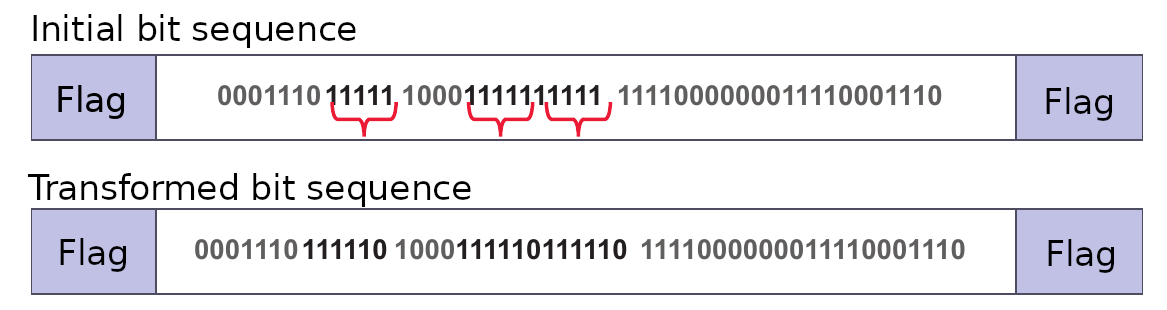
\includegraphics[scale=0.4]{images/2-16.png} 
     	%\vspace*{-0.5em}
		%\caption{Floating gate transistor cell}
	\end{figure}	
	\end{center}
	
	Here one "0" bit is added every 5 "1" bits. (because 6 "1" bits is the flag).
	 
	\end{frame}

	\subsection{Control of integrity}

	\begin{frame}
	
	It's important to ensure the received data has not bee altered (by electromagnetic disturbance, loss of synchronization, etc.).
	\vspace*{0.5em} 
	
	There are some techniques to control the integrity of the data. 
	\vspace*{0.5em}
	
	But first let's talk about the Binary Error Rate (BER):
	\vspace*{1em}
	
	$BER = \frac{number\ of\ erroneous\ bits}{number\ of\ transmitted\ bits}$
	\vspace*{0.5em}
	
	ex:
	bit word sent:     011010110101
	bit word received: 001010010101	
	\vspace*{1em}
	
	$BER=\frac{2}{12}=0.18$	
	\vspace*{0.5em}	
		
	But in reality 	the $BER$ varies from $10^{-4}$ (phone network) to $10^{-9}$ (local computer network).
	
	\end{frame}

	\begin{frame}
	
	For one bit $BER$ = probability of having erroneous bits
	$(1-BER)$ = probability of having correct bits
	\vspace*{1em}
	
	So if $BER=10^{-4}$ and we have 800 bits to transmit.
	\vspace*{1em}
	
	Probability of receiving a correct block is:
	$(1-BER)^{800}=(1-10^-4)^{800}=0.923$
	\vspace*{1em}
	
	Probability of receiving a bad block is:
	$1-0.923=0.077$	
	 	
	\end{frame}

	\begin{frame}
	
	So how to detect an error during the transmission of a block?
	\vspace*{1em}
	
	Four techniques to detect transmission errors:	
	\vspace*{1em}
	
	\begin{enumerate}
	\item{Detection using an echo}
	\item{Detection using repetition}
	\item{Detection using a computed key}
	\item{Detection and autocorrection using a code system}
	\end{enumerate}
	
	\end{frame}

	\begin{frame}
	
	Detection using a echo:
	\vspace*{1em}
	
	The receptor resend the received message. The source checks if the resent message is the same as the originally sent message.
	If not: message is send again.
	\vspace*{1em}
	
	Detection using repetition (statistical approach):
	\vspace*{1em}
	
	The source send several times the message. If all the messages are the same: no errors occurred!
	If not: a bunch of messages is sent again. 
	
	\end{frame}

	\begin{frame}
	
	Detection using a computed key:
	\vspace*{1em}
	
	A supplementary information is send within the message: a computed key. The value of this key depends on the message itself. 
	\vspace*{0.5em}
	
	The receptor can check if the transmitted key match the message. If it does not: the message is sent back.
	\vspace*{1em}
	
	Two main techniques to do that:
	\vspace*{1em}
	
	\begin{enumerate}
	\item{Parity bit technique (or VRC)}
	\item{Cyclic redundancy check technique (or CRC)}
	\end{enumerate}		
	
	
	\end{frame}

	\begin{frame}
	
	Parity bit technique:
	\vspace*{1em}
	
	The principle is the following: a bit is added at the end of the sequence of bits of the message. 
	\vspace*{0.5em}
	
	key = sum of the bits equal to 1 modulo 2 	
	
	Ex: 1001111 
	In this case we have 5 bits equal to 1. So $key=5\%2=1$
	\vspace*{1em}	
	
	\begin{block}{Note}
	Can only detect errors on impair number of bits messages. Used mainly in asynchronous transmission. For synchronous transmission a variant exists: the LRC (Longitudinal redundancy check technique) 	
	\end{block}	
	
	\end{frame}

	\begin{frame}
	
	Cyclic Redundancy Technique (CRC):
	\vspace*{1em}
	
	\begin{center}	
	\begin{figure}
		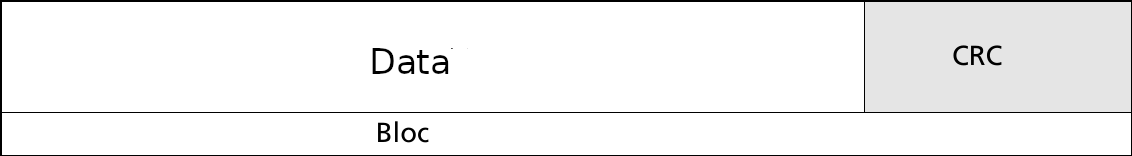
\includegraphics[scale=0.4]{images/2-18.png} 
     	%\vspace*{-0.5em}
		%\caption{Floating gate transistor cell}
	\end{figure}	
	\end{center}
	
	The CRC is deduced form a math operation applied to the data itself.
	\vspace*{0.5em}
	
	The block of data N bits is considered as a polynomial of degree N-1: P(X).
	\vspace*{0.5em}
	
	This polynomial is divided by a polynomial generator G(X) (according to boolean arithmetic).
	\vspace*{0.5em}
	The rest of the division R(X) is the CRC. The CRC is then transmitted with the block.
	\vspace*{0.5em}
	
	The transmitted CRC is compared to the received CRC: if not equal there is an error!
	
	\end{frame}

	\begin{frame}
	
	We perform $\frac{(P(X) + R(X))}{G(X)}$ if it is equal to 0, then the message is OK!
	
	\begin{block}{Note}
	In boolean arithmetic, addition and subtraction are equivalent $P(X)-R(X) \equiv P(X)+R(X)$
	
	\end{block}
	\vspace*{1em}
	
	Example: we want to protect the message 110111 using a polynomial $G(x)=x^2+x+1$
	\vspace*{0.5em}
	
	110111 => $P(x) = x^5+x^4+0\times x^3+x^2+x^1+x^0$ 
	\vspace*{0.5em}
	
	In order to allow the addition of the message and the key we multiply $P(x)$ by $x^m$ (with m = degree of the generator polynomial) so we have: $P(x)\times x^2= x^7+x^6+0\times x^5+x^4+x^3+x^2$.
	\vspace*{0.5em}
	
	\end{frame}
	
	\begin{frame}	
	
	\begin{center}	
	\begin{figure}
		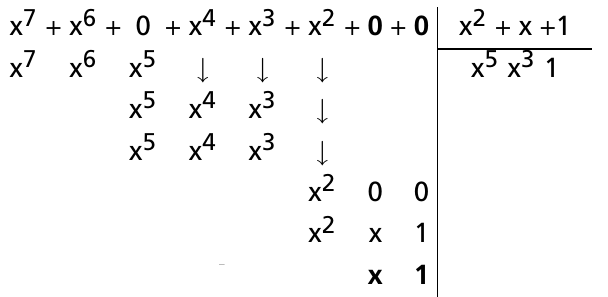
\includegraphics[scale=0.5]{images/2-17.png} 
     	%\vspace*{-0.5em}
		%\caption{Floating gate transistor cell}
	\end{figure}	
	\end{center}		
	
	$P(x)\times x^2$ divided by $G(X)$ give a rest $R(x)=X+1$ (so the CRC=11).
	\vspace*{0.5em}
	
	So the block to transmit is now the following: 11011111
	\vspace*{0.5em}
	
	\begin{block}{Note}
	The best generator polynomial is a tradeoff ensuring:
	\begin{itemize}
	\item{a low probability of non-detection}
	\item{not penalizing too much the transmission}
	\end{itemize}
	\end{block}	 
		
	
	\end{frame}

	\begin{frame}
	
	Detection and auto-correction using a code system:
	\vspace*{1em}
	
	Original binary words are substituted  by new binary words with auto-correcting capacities.
	\vspace*{1em}
	
	\begin{center}	
	\begin{figure}
		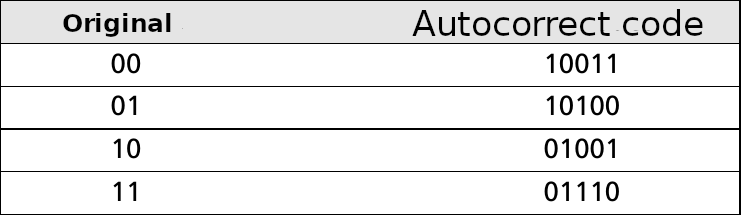
\includegraphics[scale=0.4]{images/2-19.png} 
     	%\vspace*{-0.5em}
		%\caption{Floating gate transistor cell}
	\end{figure}	
	\end{center}	
	
	Let's imaging we transmit the binary word 10011. And let's imaging the receptor receives the binary word with one bit wrong. So it can be: 10011 10001 10111 11011 or 00011.\vspace*{1em}
	
	
	None of these codes match 10011 but for all theses cases the closest code is 10011 (Hamming distance = 1 with this one!)
	
		
	\end{frame}

	\section{Exchange control}
	\subsection{Send and wait approach}

	\begin{frame}
		
	With the send and wait approach the source sends a block to the receptor. 
	
	\begin{center}	
	\begin{figure}
		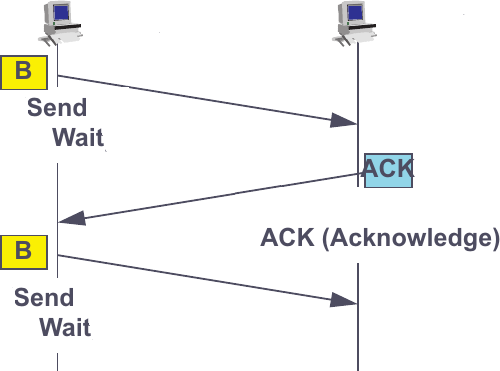
\includegraphics[scale=0.5]{images/2-20.png} 
     	%\vspace*{-0.5em}
		%\caption{Floating gate transistor cell}
	\end{figure}	
	\end{center}	
		
	Once received the receptor sends back ACK (to tell it it can receive the next block). The source waits a certain amount of time this ACK. 
	
	\vspace*{1em}
	If it does not receive it, it sends again the block (Re-transmission Time Out). 	 
	
	\end{frame}

	\begin{frame}
	
	But if ACK is lost, the same block is sent again ... 
	
	\begin{center}	
	\begin{figure}
		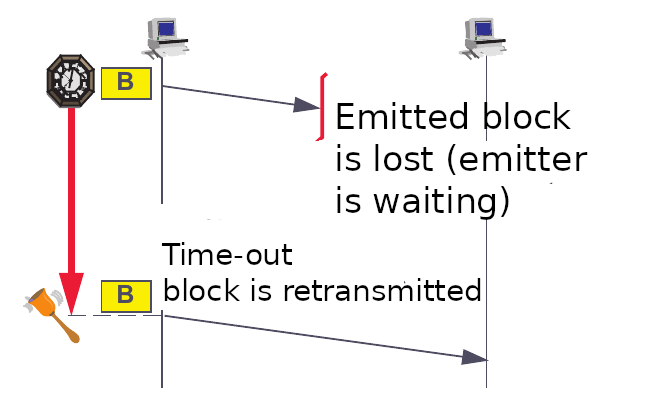
\includegraphics[scale=0.38]{images/2-21.png} 
     	%\vspace*{-0.5em}
		%\caption{Floating gate transistor cell}
	\end{figure}	
	\end{center}	
	
		
	To avoid duplication, each block has a number N. If the block N=1	has already been received, a new block N=1 will not be added after ...	 In order to avoid re-transmission conflicts.

	\begin{center}	
	\begin{figure}
		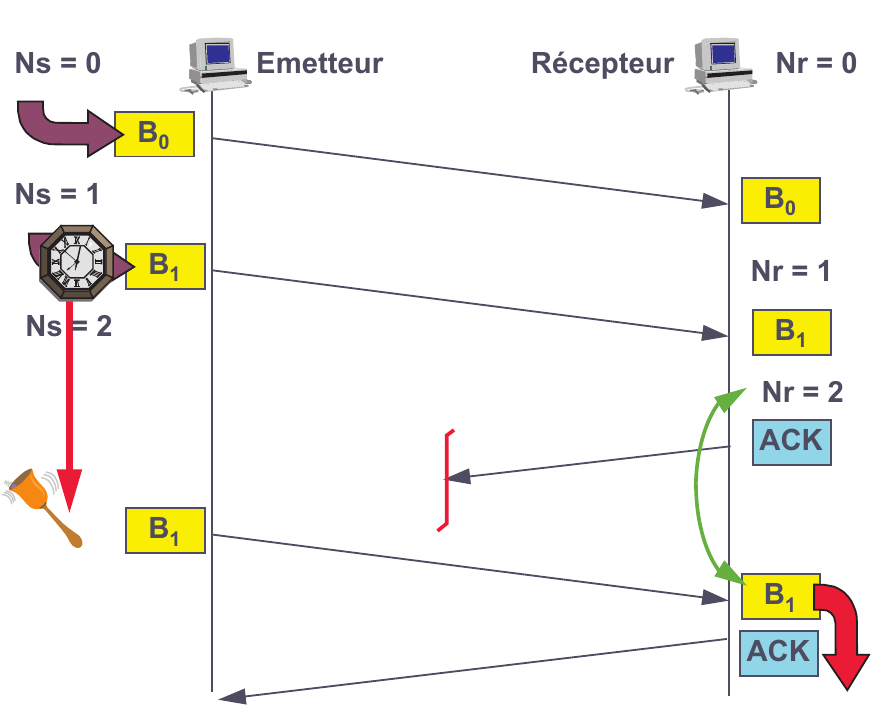
\includegraphics[scale=0.28]{images/2-22.png} 
     	%\vspace*{-0.5em}
		%\caption{Floating gate transistor cell}
	\end{figure}	
	\end{center}	

	ACKs are also numerated in practice.

	\end{frame}
	
	\subsection{Anticipation approach}

	\begin{frame}

	In this case all the blocks are sent one after the other, without waiting for the first ACK. 

	\begin{center}	
	\begin{figure}
		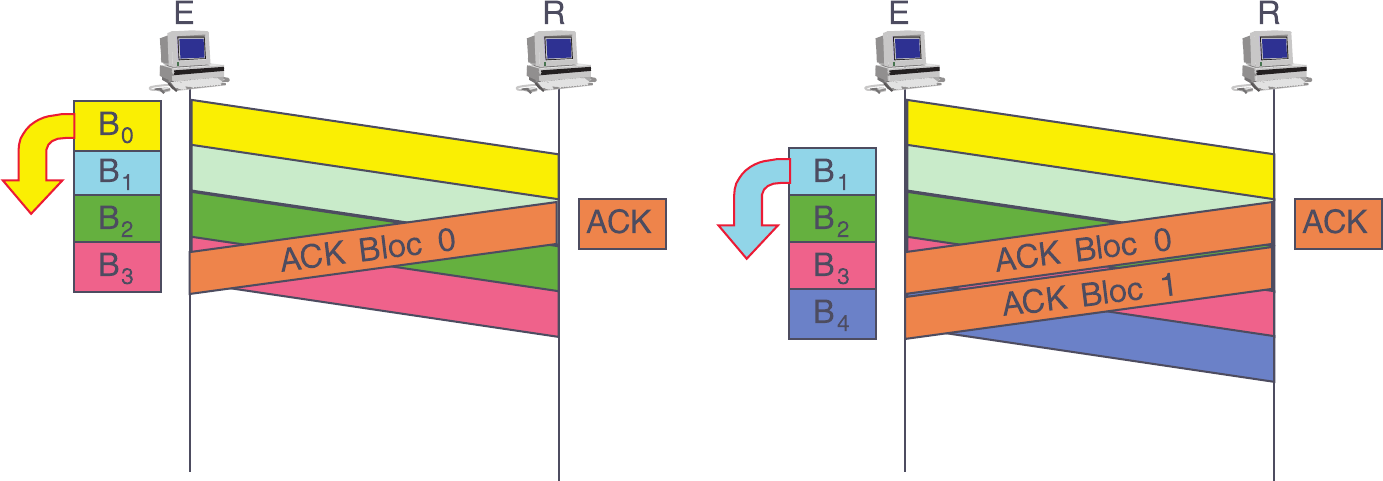
\includegraphics[scale=0.28]{images/2-23.png} 
     	%\vspace*{-0.5em}
		%\caption{Floating gate transistor cell}
	\end{figure}	
	\end{center}
	
	Blocks can also be acknowledged by groups, for further optimization. 	With this approach, the transfer is optimized.
		
	\begin{center}	
	\begin{figure}
		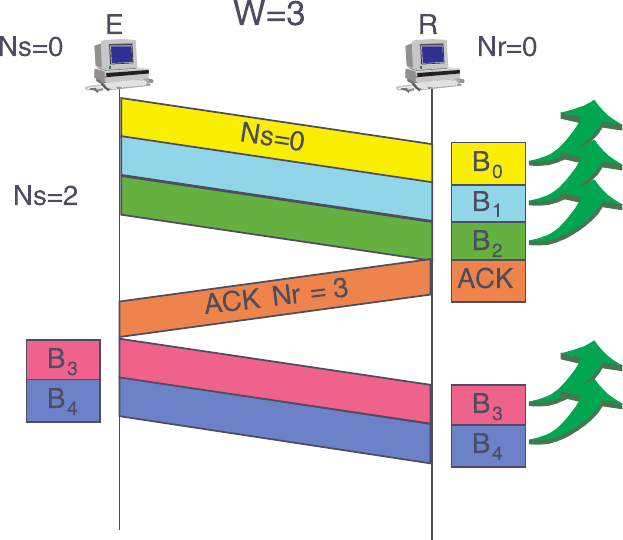
\includegraphics[scale=0.28]{images/2-24.png} 
     	%\vspace*{-0.5em}
		%\caption{Floating gate transistor cell}
	\end{figure}	
	\end{center}
	
	W: window of anticipation, number of blocks the emitter can memorize waiting for acknowledgment 	(ACKs).	
	
	\end{frame}
	
	\begin{frame}
	
	In case of transmission errors, two techniques:
	\vspace*{1em}
	
	\begin{enumerate}
	\item{the bad block is rejected and block is re-transmitted}
	\item{the group of blocks is rejected and all the blocks are re-transmitted}
	\end{enumerate}
	\vspace*{1em}
	
	The first approach is the selection rejection. The transmission is optimized but it requires bigger memory (other blocks of the group need to be kept in memory). And blocks need to be re-ordered by the receptor (requires computation power).\vspace*{0.5em}
	
	With the second approach the memory is optimized and the computation power of the receptor is minimized (no need to reorder the blocks!).	
	
	\end{frame}

	\subsection{Flux control}

	\begin{frame}
	
	During a transmission, the receptor has a certain number of free slots in its buffer (memory).
	\vspace*{0.5em}
	
	Because the receptor has also other tasks to realize, not all the memory may be available and some blocks may be lost!\vspace*{0.5em}
	
	That's why it's important to control the emitting cadence of the source.\vspace*{1em}
	
	\begin{center}	
	\begin{figure}
		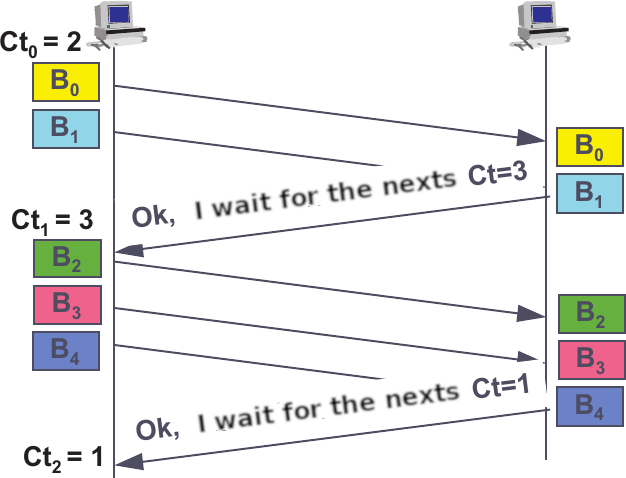
\includegraphics[scale=0.5]{images/2-25.png} 
     	%\vspace*{-0.5em}
		%\caption{Floating gate transistor cell}
	\end{figure}	
	\end{center}

	\end{frame}

	\subsection{Control of the link (or signalization)}
	
	\begin{frame}
	
	Before transmitting any data it is necessary to make a link between the two computers. And once the transmission is finished, the link is closed.\vspace*{1em}
	
	To manage this link we send signalization information (transmitting through the same channel as the data). Sometimes the signalization information is sent through its own channel.\vspace*{0.5em}	
	
	\begin{center}	
	\begin{figure}
		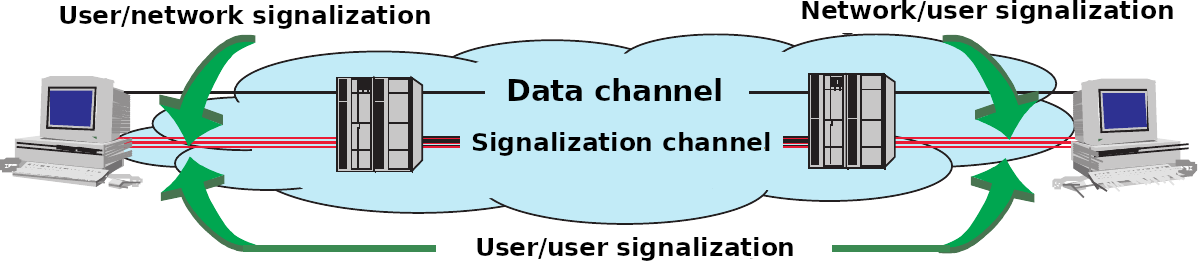
\includegraphics[scale=0.5]{images/2-26.png} 
     	%\vspace*{-0.5em}
		%\caption{Floating gate transistor cell}
	\end{figure}	
	\end{center}	
	
	\end{frame}




\end{document}